\section{Concept}

Based on the initial idea to somehow move from a dense point cloud to a 3D mesh that can be used in the 3D graphic suite Blender, it was important to plan ahead.\\
When looking at previous research papers (references?) some approaches try to solve problems by applying a transformation of some sort to the original state to get a modified one, which reminds of how the Pellerhaus changed during the last 400 years.\\
It is possible to mesh a 3d point cloud with several algorithms by trying to find the nearest neighbour of a point in 3d space. One such algorithm is called Delaunay Tetrahedralization  (see: http://www.cs.berkeley.edu/~jrs/papers/cdtbasic.pdf) and is used in the free multi-view reconstruction software "Visual SFM", for instance.\\
With our method we try to utilize the characteristics of laser scanners in such a way, that we know every aquired point can be described by scaling and rotating a unit sphere. In mathematical terms we can determine the spherical coordinates of every point in our point cloud. The 3d points need to be converted from their cartesian coordinate system to the spherical coordinate system first (see  http://en.wikipedia.org/wiki/Coordinate\_system). Using this simple principle we can not only mesh a point cloud generated by a laser scanner, we can texture it, too. With the coordinates ranging from 0 to 360 degrees horizontally, 0 to 180 degrees vertically and a depth coordinate ranging from 0 to the maximum scan distance we are able to create two images, namely a depth map and a color map. Those images are then being used to create a regular grid which is used for meshing and texture coordinates. By applying the inverse transform to the spherical coordinates it is possible to get the model in cartesian space and export it to any 3d file format. This process is explained in more detail in this chapter.\\
Furthermore it was neccessary to know how the user will be operating with the software. Usually a use case diagram is created to determine the required functions the software must provide in order to let a user accomplish his desired goals.

\pagebreak

\subsection{Use case diagram}

\begin{figure}[h]
	\centering
	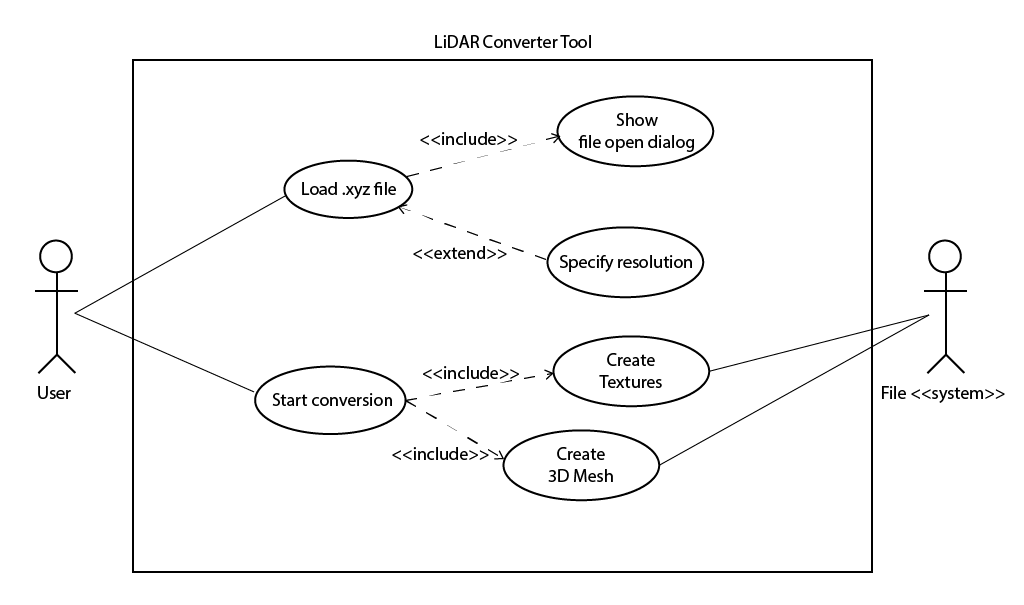
\includegraphics[scale=0.4]{UseCaseDiagram_PC2B.png}
	\caption{Use Case Diagram}
	\label{fig:use_case}
\end{figure}


\subsection{Laser scanning on location}

For data aquisition we used the Faro Focus 3D laser scanner on the 21.1.2015 16:39:15. First, the device should be configured by setting e.g. the desired resolution (for scan and photos), maximum scan distance (which results in a change of the eye-safety distance), a project name and GPS location (if no GPS module is available like in our case). This configuration can be done in the office or on-site. After the device was set up, the scan process was started. During scanning the main body rotates horizontally and a mirror mounted inside the body rotates vertically. This creates the uncolored point cloud. After the scanning process, several pictures are taken by the built-in camera to color the point cloud. Beforehand the scanner measures the exposure to avoid under- or overexposured photographs. Finally, the inclination is measured with an inclinometer to level the point cloud properly.
This procedure was repeated five times to get additional scans covering viewpoints that have been obstructed by obstacles.

While scanning a site we faced problems we didn't expect. We encountered people randomly walking in the laser beam (resulting in vertical lines in the final scan), a suprisingly occuring crash of the device's operating system leading to a terminal output (wrecking the sd card with all previous scans) and a man asking if we took a photo of him while he was entering the building(?!).


\begin{figure}[h]
	\centering
	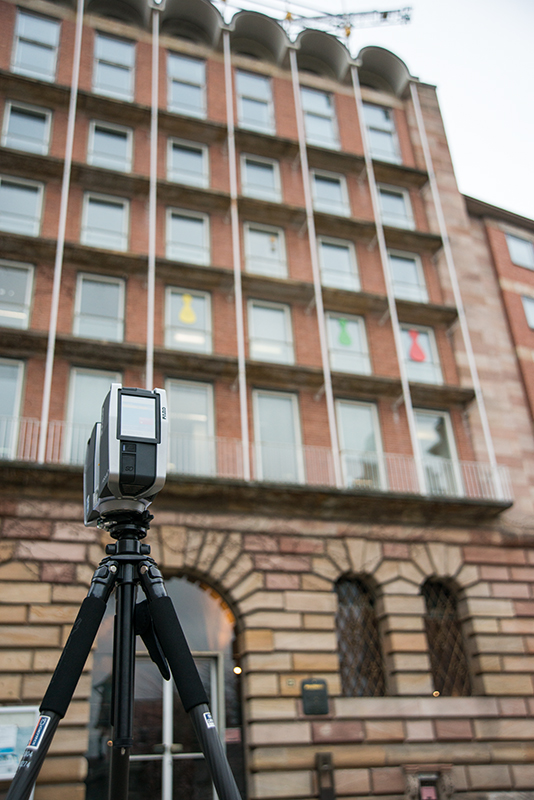
\includegraphics[scale=0.4]{PellerhausLaserScan.jpg}
	\caption{Scanning with Faro Focus 3D}
	\label{fig:laser_scanning_on_location}
\end{figure}



\begin{table}[h]
	\centering
	\begin{tabular}{l | l | l}
		A & B & C \\
		\hline
		1 & 3 & 4 \\
		1 & 3 & 4 \\
	\end{tabular}
	\caption{very basic table caption}
	\label{tab:abc}
\end{table}

\pagebreak


\section{Generating data and testing algorithms}

\subsection{BlenSor}

The Blender Sensor Simulation Toolbox (compare \parencite{Gschwandtner11b}) is a custom version of the open source software Blender allowing to simulate different types of scanning within a virtual 3d scene. It is being developed by the Department of Computer Sciences, University of Salzburg, Austria. The goal of this project is to provide a tool, mostly aimed at researchers, that can help with testing algorithms for fields such as obstacle detection and tracking, range data segmentation or surface reconstruction.\\
We found this software very useful to begin with the development of PC2B. With a number of scanner presets it is possible to generate a point cloud of the virtual environment from different types of scanner devices.

\subsection{Test-Addon for Blender}

During the beginning of the software development process the point cloud projection didn't seem to be correct. Testing the algorithm responsible for projecting from cartesian to spherical coordinates was very tedious, because it involved importing the files, waiting for the images to get generated and then either look at the image files to find mistakes or continue with the meshing process. This pipeline was prone to errors which might affect the result.\\
Hence, a custom addon for Blender was developed to test the algorithm for the correct mathematics. The language used for addons is Python 3 and enables for developing powerful extensions to the Blender core.

A more efficient approach would be to develop a new modifier in C/C++ that integrates directly into Blender. Unfortunately diving into Blender Core Development is not very easy due to its huge code base. In addition the time constraint didn't permit experimenting with this approach.


\section{Prototype}

The working title of the converter software was defined as "PointCloud2Blender", PC2B in short, because this was the main goal of the software project.

\subsection{Point Cloud Importer}

A crucial part of the PC2B converter software is the ability to import point clouds saved as files. There is a huge amount of file types that can accomodate such a data structure. Points can be stored in ASCII or Binary form. Importing binary formats requires to know the exact structure of the file and the bytes used for certain values. Documentation was limited for many of the file formats, so using ASCII files was a better choice from the beginning. Initially it was planned to only import the .xyz file format, since this is a very simple file format that can be exported in ASCII form from the proprietary Faro SCENE 5 software which is needed for preprocessing the raw point cloud stream produced by the Faro Focus 3D.\\
During development it turned out that support for the .ply file format is desirable, since scientific websites that provide models (see) widely provide this file type. Also Blender can export a 3D model to this file format. This fact was extremly useful for testing the algorithm, which is described later.

\subsubsection{Point Cloud data formats}

Working with such file structures like in our case is very easy. See \ref{tab:xyz_ply_file_structure}.


\begin{table}[h]
	\centering
	\begin{subtable}[b]{0.46\textwidth}
		
		\resizebox{\textwidth}{!}{%
		\begin{tabular}{l}
			-59.43620000 -31.36650000 302.80950000 59 46 55 \\
			-60.34600000 -31.80190000 302.85280000 58 45 54 \\
			-60.51810000 -31.88870000 302.71900000 58 45 54 \\
			-59.50470000 -31.39880000 302.68240000 56 47 50 \\
			-60.32350000 -31.79130000 302.89580000 59 46 54 \\
			-59.40940000 -31.35360000 302.85200000 61 48 57 \\
			-67.58220000 -29.73320000 302.12780000 73 55 58 \\
			-67.51000000 -29.59980000 302.04520000 63 43 54 \\
			-66.18880000 -29.78650000 299.88830000 100 87 80 \\
			-67.54620000 -29.66590000 302.08650000 64 47 56 \\
			-67.50660000 -29.59690000 302.00010000 62 43 51 \\
			-67.51970000 -29.60540000 302.09000000 64 46 57 \\
			...
		\end{tabular}}
		\caption{Sample .xyz file}
		\label{tab:xyz_file}
	\end{subtable}
	\hfill
	\begin{subtable}[b]{0.52\textwidth}
		\resizebox{\textwidth}{!}{%
		\begin{tabular}{l}
			ply \\
			format ascii 1.0 \\
			comment VCGLIB generated \\
			element vertex 2900882 \\
			property float x \\
			property float y \\
			property float z \\
			property uchar red \\
			property uchar green \\
			property uchar blue \\
			property uchar alpha \\
			element face 0 \\
			property list uchar int vertex\_indices \\
			0.480478 -0.877007 0.000000 -0.479092 0.877764 0.000000 \\
			0.477702 -0.878522 0.000000 -0.479092 0.877764 0.000000 \\
			0.477702 -0.878522 0.661730 -0.479092 0.877764 0.000000 \\
			0.480478 -0.877007 0.661730 -0.479092 0.877764 0.000000 \\
			-0.373352 0.927690 0.000000 0.371881 -0.928280 0.000000 \\
			-0.370417 0.928866 0.000000 0.371881 -0.928280 0.000000 \\
			-0.370417 0.928866 0.661730 0.371881 -0.928280 0.000000 \\
			-0.373352 0.927690 0.661730 0.371881 -0.928280 0.000000 \\
			0.110288 0.993900 0.000000 -0.111863 -0.993724 0.000000 \\
			0.113431 0.993546 0.000000 -0.111863 -0.993724 0.000000 \\
			0.113431 0.993546 0.661730 -0.111863 -0.993724 0.000000 \\
			0.110288 0.993900 0.661730 -0.111863 -0.993724 0.000000 \\
			...
			
		\end{tabular}}
		\caption{Sample .ply file}
		\label{tab:ply_file}
	\end{subtable}
	\caption{Sample generated point cloud files}
	\label{tab:xyz_ply_file_structure}
\end{table}

\subsection{Determine original point cloud resolution}

Users of PC2B have the option to determine the resolution of the 3D panorama. It can either be set to fixed multiples of 360 by 180 pixels or set to a custom resolution. We have implemented an algorithm to help the user find the best resolution for his particular point cloud. It works as follows:

\subsection{Projecting 3D points onto a 2D plane}

This is inside the text $\cos (2\theta) = \cos^2 \theta - \sin^2 \theta$.


And this is a separate formula:
$$\cos (2\theta) = \cos^2 \theta - \sin^2 \theta$$


\subsection{Saving textures}

The generated depth and color maps are stored with 8-bit unsigned integer values ranging from 0 to 255. After the file has been imported they can be saved directly as .jpg image files.

\subsection{OpenGL Point Cloud Viewer}

This russian video tutorial was very helpful with the basic setup with the Qt framework.

\cite{ytQtOpenGL}

\subsection{Meshing}

Using the current pixel inside two for-loops in combination with the neighboring pixels to the right, bottom-right and bottom makes up a quad, which can be textured.

\subsection{Texture Coordinates and Normals}

Texture Coordinates go from 0.0 to 1.0 in the x and y direction, respectively. Usually the texture coordinate axes are referred to as s and t. By dividing the current coordinate by the width and the height of the image, respectively, the coordinates can be normalized.

Calculating normals is accomplished by using the cross product of the two vectors forming the current quad.

\subsection{Mesh Exporter}

There are different formats, one had to be chosen that supported at least vertices and faces.

\subsubsection{.obj}

The .obj format is the most popular and can be one of the easiest to understand file formats to save 3D geometry with not only points, but vertices, normals, texture coordinates and much more. It was the first choice when testing mesh exporting from the converter software and examining it in Blender.

\subsubsection{.blend}

A personal goal for this research was to implement a .blend export feature to allow for a native importing of the panorama mesh into Blender. However, this goal was not reached in this project. As it turned out, exporting the binary Blender file format was quite complicated, due to it's versatile structure. An experienced Blender Developer, Jeroen Bakker, stated in 2009 “When implementing loading and saving blend-files in a custom tool the difficulty is the opposite. In a custom tool loading a blend-file is easy, and saving a blend-file is difficult.” \parencite[see]{webMysteryOfTheBlend}. At least implementing it with the limited time for the thesis it was not feasable.



\subsubsection{custom format}

Even the Blender community suggested to not use the .blend format directly, but rather try a custom binary format. \parencite[compare]{webBlenderArtistsBlendExport}


\subsection{Optimizations}

The initial algorithms and approaches had some flaws, which needed to get eliminated to get a clean mesh out of the converter. Those are presented as follows:

\subsubsection{Flip horizontal direction of panorama}

The panorama is flipped horizontally.

\subsubsection{Panorama pixel depth testing}

It can happen that two points from the point cloud happen to result in the same pixel in the 2D panorama. This might result in a noisy image result, if not handled with care. To avoid any errors, it is important to take only the closest point to the camera, instead of letting every point override the corresponding pixel in the image.

\subsubsection{Panorama noise reduction}

Since there is only a limited number of points, the panorama texture gets quite noisy, especially with a higher resolution option set in the converter. A harsh change from light gray to black values in the depth map will result in a noisy 3D structure as well.
To solve this issue, the image is blurred by a user setting or automatically (TODO!).

\subsubsection{Remove doubles}

The meshing technique resulted in a very high point count for the .obj file. Example: For a 4x resolution panorama with 2,198,528 vertices, using the "remove doubles" option in Blender 3D automatically removed 2,100,716 vertices.
Solution: several passes for vertices, texture coordinates and normals (TODO!).

\subsubsection{3D Distortion}

The generated 3D mesh from the 2D panorama results in a distorted one, the more it touches the top.
Solution: None yet.

\subsubsection{Tiling}

Due to the higher resolution meshes having several megabytes in size and taking some time to import in Blender, this has to be optimized somehow.
Solution: Create tiles when higher resolution is set. E.g. with a 4x resolution, create four tiles (that's four seperate .obj files).